Consider the polynomial $x^n-1 \in \Q[x]$. Consider the $n^{\text{th}}$-roots of unity
$$U_n = \set{\alpha \in \C : \alpha \text{ is a root of } x^n-1}$$
A nonzero complex number $a+bi \in \C$ can be written uniquely in the form
$$r(\cos \theta + i \sin \theta) = re^{i\theta},~~r > 0,~~0 \leq \theta < 2 \pi$$
So, the roots of $x^n - 1$ are of the form 
$$e^{\frac{2\pi i k}{n}} = \cos \left(\frac{2\pi k}{n}\right) + i\sin \left(\frac{2\pi k}{n}\right), ~~k = 0,1,2,...,n-1$$
Notice that 
$$\left(e^{\frac{2\pi i k}{n}}\right)^n = e^{2\pi i k} = \cos(2\pi k) + i\sin(2\pi k) = 1$$
So we have that $e^{\frac{2\pi i k}{n}}$ is a root of $x^n -1$. Geometrically, $e^{\frac{2\pi i k}{n}}$ are equally spaced points on the unit circle in the complex plane starting at $(1,0)$.

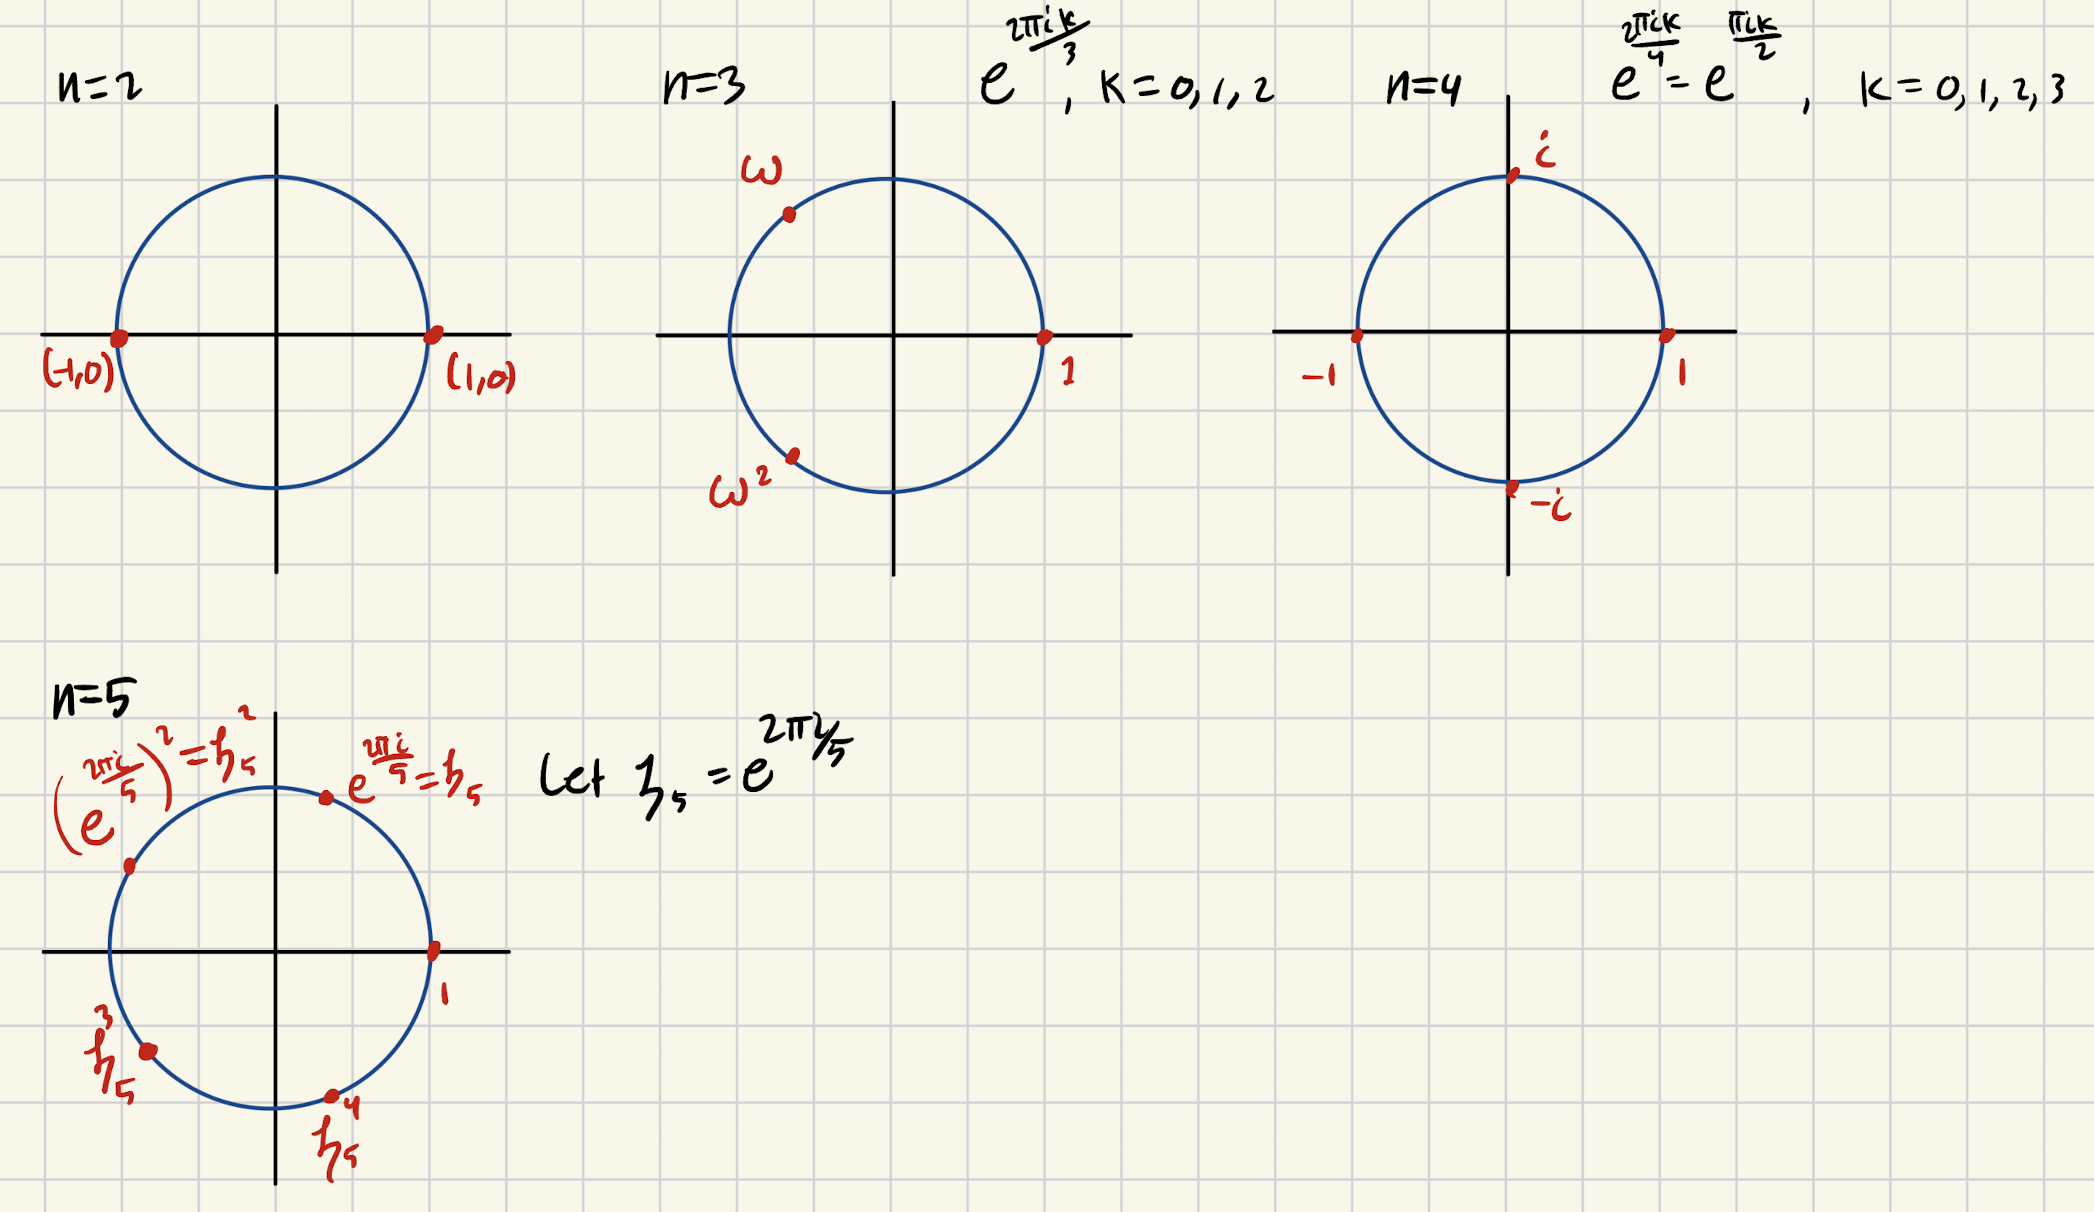
\includegraphics[width = 400pt, center]{CH4/images/Roots of Unity Circles.png}

Since $x^n - 1$ has at most $n$ roots in $\C$, it follows that all of the roots of $x^n -1$ are of the form $e^{\frac{2\pi i k}{n}}$ for $k = 0,1,..., n-1$. It's pretty easy to show $U_n$ is a group with respect to multiplication by constructing the following isomorphism:
\begin{align*}
    \quotient{\Z}{n\Z} &\to U_n \\
    k &\mapsto \left(e^{\frac{2 \pi i}{n}}\right)^k
\end{align*}
which would give us that $e^{\frac{2\pi i}{n}}$ is cyclic.

\begin{definition}[Primitive Root of Unity] \leavevmode \\
    A generator of $U_n$ is called a primitive root of unity.
\end{definition}

Let $\zeta$ be a primitive $n^\text{th}$-root of unity. Then
$$|\zeta |^k = \frac{n}{\gcd(n,k)}$$
Since $k = 0,1,...,n-1$, there are exactly $\phi(n)$ primitive $n^\text{th}$-roots of unity. Let $\zeta_n = e^{\frac{2\pi i}{n}}$. Some useful roots to know:
\begin{align*}
    \zeta_1 &= 1 \\
    \zeta_2 &= -1 \\
    \zeta_3 &= -\frac{1}{2} + \frac{\sqrt{3}}{2}i \\
    \zeta_4 &= i \\
    \zeta_5 &= \frac{\sqrt{5}-1}{4} + \frac{\sqrt{10+2\sqrt{5}}}{4}i \\
    \zeta_6 &= \frac{1}{2} + \frac{\sqrt{3}}{2}i \\ 
    \zeta_7 &= e^{\frac{2\pi i}{7}} \\
    \zeta_8 &= \frac{1}{\sqrt{2}} + \frac{1}{\sqrt{2}}i
\end{align*}

\begin{definition}[Cyclotomic Field] \leavevmode \\
    The field $\Q(\zeta_n)$ is called the cyclotomic field of $n^\text{th}$-roots of unity.
\end{definition}

Let $p$ be a prime.
\begin{align*}
    [\Q(\zeta_p) : \Q] &= p-1 \\
    x^p - 1 &= (x-1)(x^{p-1}+x^{p-2} + ... + x + 1) \\ 
    \implies \frac{x^p-1}{x-1} &= x^{p-1}+x^{p-2} + ... + x + 1
\end{align*}

We proved that $p(x) = \frac{x^p-1}{x-1}$ is irreducible ($p(x+1)$ with Eisenstein's Criterion). Since $\zeta_n \neq 1,$ $n > 1$ where $\zeta_n$ is a root of $p(x)$, so $m_{\zeta_n, \Q}(x) = p(x)$. In general,
$$[\Q(\zeta_n) : \Q] = \phi(n)$$

\begin{example}
    Find splitting field of $x^p - 2 = f(x) \in \Q[x]$, where $p$ is a prime. Note that the solutions to $f(x)$ are 
    $$\sqrt[p]{2} \zeta_p^k \text{ for } k= 0, 1, ..., p-1$$
    Let $K$ be the splitting field of $f(x)$ over $\Q$.
    $$K = \Q\left(\sqrt[p]{2}, \sqrt[p]{2}\zeta_p, \sqrt[p]{2}\zeta_p^2, ..., \sqrt[p]{2}\zeta_p^{p-1}\right)$$
    We know that $\sqrt[p]{2}, \sqrt[p]{2}\zeta_p \in K$. This implies
    $$\dfrac{\sqrt[p]{2}\zeta_p}{\sqrt[p]{2}} = \zeta_p \in K$$
    So, $K$ contains $\Q, \sqrt[p]{2}, \zeta_p$, so it contains $\Q(\sqrt[p]{2},\zeta_p)$. Note that since all the roots of $f(x)$ are of the form $\zeta_p^k \sqrt[p]{2},$ we have that all of $f(x)$'s roots are in $\Q(\sqrt[p]{2},\zeta_p)$. Hence
    $$K\subseteq \Q(\sqrt[p]{2},\zeta_p)$$
    So $K = \Q(\sqrt[p]{2},\zeta_p)$ and
    $$[K : \Q] = [K : \Q(\sqrt[p]{2})][\Q(\sqrt[p]{2}): \Q] \leq (p-1)p$$
    and $p \mid [K : \Q]$. Similarly, $p-1 \mid [K : \Q]$. Since $\gcd(p-1,p) = 1,$ we have that $p(p-1) \mid [K : \Q]$. Hence, $[K : \Q] = p(p-1)$.
\end{example}